%!TEX root = ../thesis.tex
%*******************************************************************************
%*********************************** Experiment *****************************
%*******************************************************************************

\chapter{Experiment} 

\ifpdf
    \graphicspath{{chapter-experiment/Figs/Raster/}{chapter-experiment/Figs/PDF/}{chapter-experiment/Figs/}}
\else
    \graphicspath{{chapter-experiment/Figs/Vector/}{chapter-experiment/Figs/}}
\fi

One of Europe's first joint ventures in science~\cite{About:1997225}, CERN (Conseil Européen pour la Recherche Nucléaire) is the largest physics research facility in the world, bringing together more than \num[group-separator={,}]{12200} people from of 110 nationalities to work together and push the frontiers of science and technology. Located at the Franco-Swiss border near Geneva, CERN was founded in 1954 and nowadays counts 23 member states~\cite{About:1997225}. CERN's main research area is particle physics, hence why the organization operates a full complex of particle accelerators and detectors.

This chapter introduces the Large Hadron Collider (LHC), CERN's main particle accelerator, as well as the ATLAS experiment, in which the SUSY search presented in this work is embedded in.

\section{The Large Hadron Collider}\label{sec:lhc}

The LHC~\cite{Evans:1129806} is the largest particle accelerator situated at CERN. It is installed in a tunnel with $\SI{26.7}{\km}$ circumference, that was originally constructed from 1984 to 1989 for the Large Electron Positron (LEP) accelerator. The tunnel is situated on the Franco-Swiss border and wedged between the Jura mountains and lake Léman. It lies between $\SI{45}{\meter}$ (in the limestone of the Juar) and $\SI{170}{\meter}$ (in molasse rock) below the surface, resulting in a tilt of $1.4\%$ towards the lake.  While proton-proton ($pp$) collisions are the main operating mode of the LHC, its design also allows it to accelerate and collide heavy ions like lead and xenon. As a particle-particle collider, the LHC obviously consists of two rings with counter-rotating beams, as opposed to particle-antiparticle colliders that only need a single ring. With an inner diameter of only $\SI{3.7}{\meter}$, the tunnel however simply too narrow to fit two separate proton rings. Instead the LHC is built in a twin bore design\footnote{Originally proposed by John Blewett at BNL for cost-saving measures of the Colliding Beam Accelerator~\cite{Evans:1129806}.}, housing two sets of coils and beam channels in a single magnetic and mechanical structure and cryostat~\cite{Evans:1129806}. While saving costs, this design has the disadvantage of both beams being magnetically coupled, thereby reducing flexibility of the machine. The LHC is composed of eight straight sections and eight arcs.

The eight straight sections each serve as interaction points (IP), either for particle detectors, or for machine hardware of the collider itself. The IPs are labelled clockwise, with IP 1 being closest to the CERN Meyrin site. Four of the eight IPs house the main particle physics experiments at the LHC, called ATLAS, CMS, ALICE and LHCb, covering a wide range of fundamental research. The two general purpose particle detectors ATLAS~\cite{Aad:2008zzm} and CMS~\cite{Chatrchyan:2008aa} are installed at IP 1 and IP 5, respectively. Both ATLAS and CMS are designed to perform high precision SM measurements including Higgs measurements as well as searches for BSM physics. Being very similar in terms of targeted phase space, ATLAS and CMS can be used to cross-check results of each other. ALICE~\cite{Aamodt:2008zz} is situated at IP 2 and specializes on heavy ion physics, studying the physics of quark-gluon plasma at high energy densities. Built in IP 5, LHCb~\cite{Alves:2008zz} targets $B$-physics and performs measurements of CP-violation. Apart from the four main experiments, three smaller experiments exist at the LHC: TOTEM, MoEDAL and LHCf. While TOTEM~\cite{Anelli:2008zza} and LHCf~\cite{Adriani:2006jd} study forwards physics close to CMS and ATLAS, respectively, MoEDAL~\cite{Pinfold:2009oia} searches for magnetic monopoles.

The eight arcs house a total of 


\begin{figure}
	\centering    
	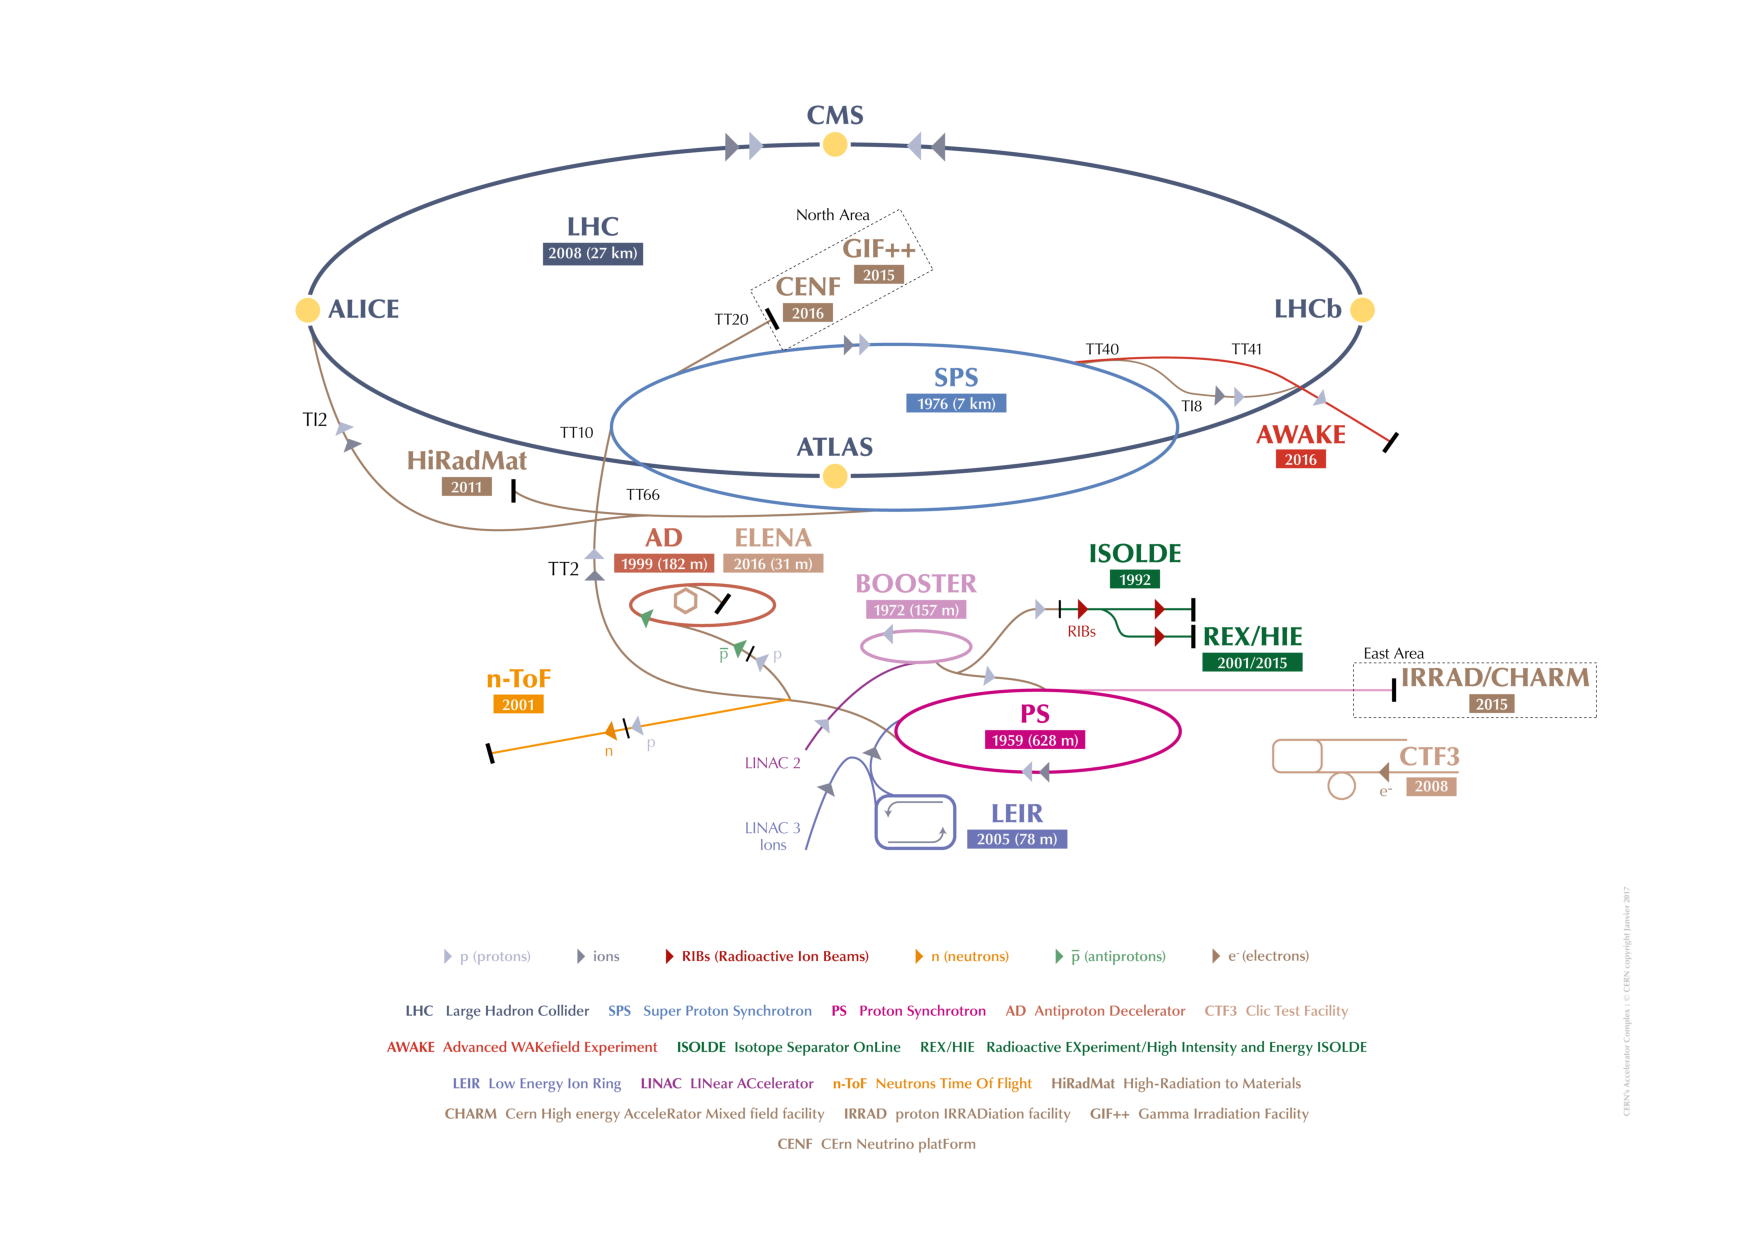
\includegraphics[width=0.9\textwidth]{CCC-v2017-noalpha}
	\caption[CERN accelerator complex]{CERN accelerator complex as of 2018~\cite{Mobs:2197559}.}
	\label{fig:accelerator_complex}
\end{figure}


\section{ATLAS Experiment}\label{sec:atlas_experiment}


\begin{figure}
	\centering    
	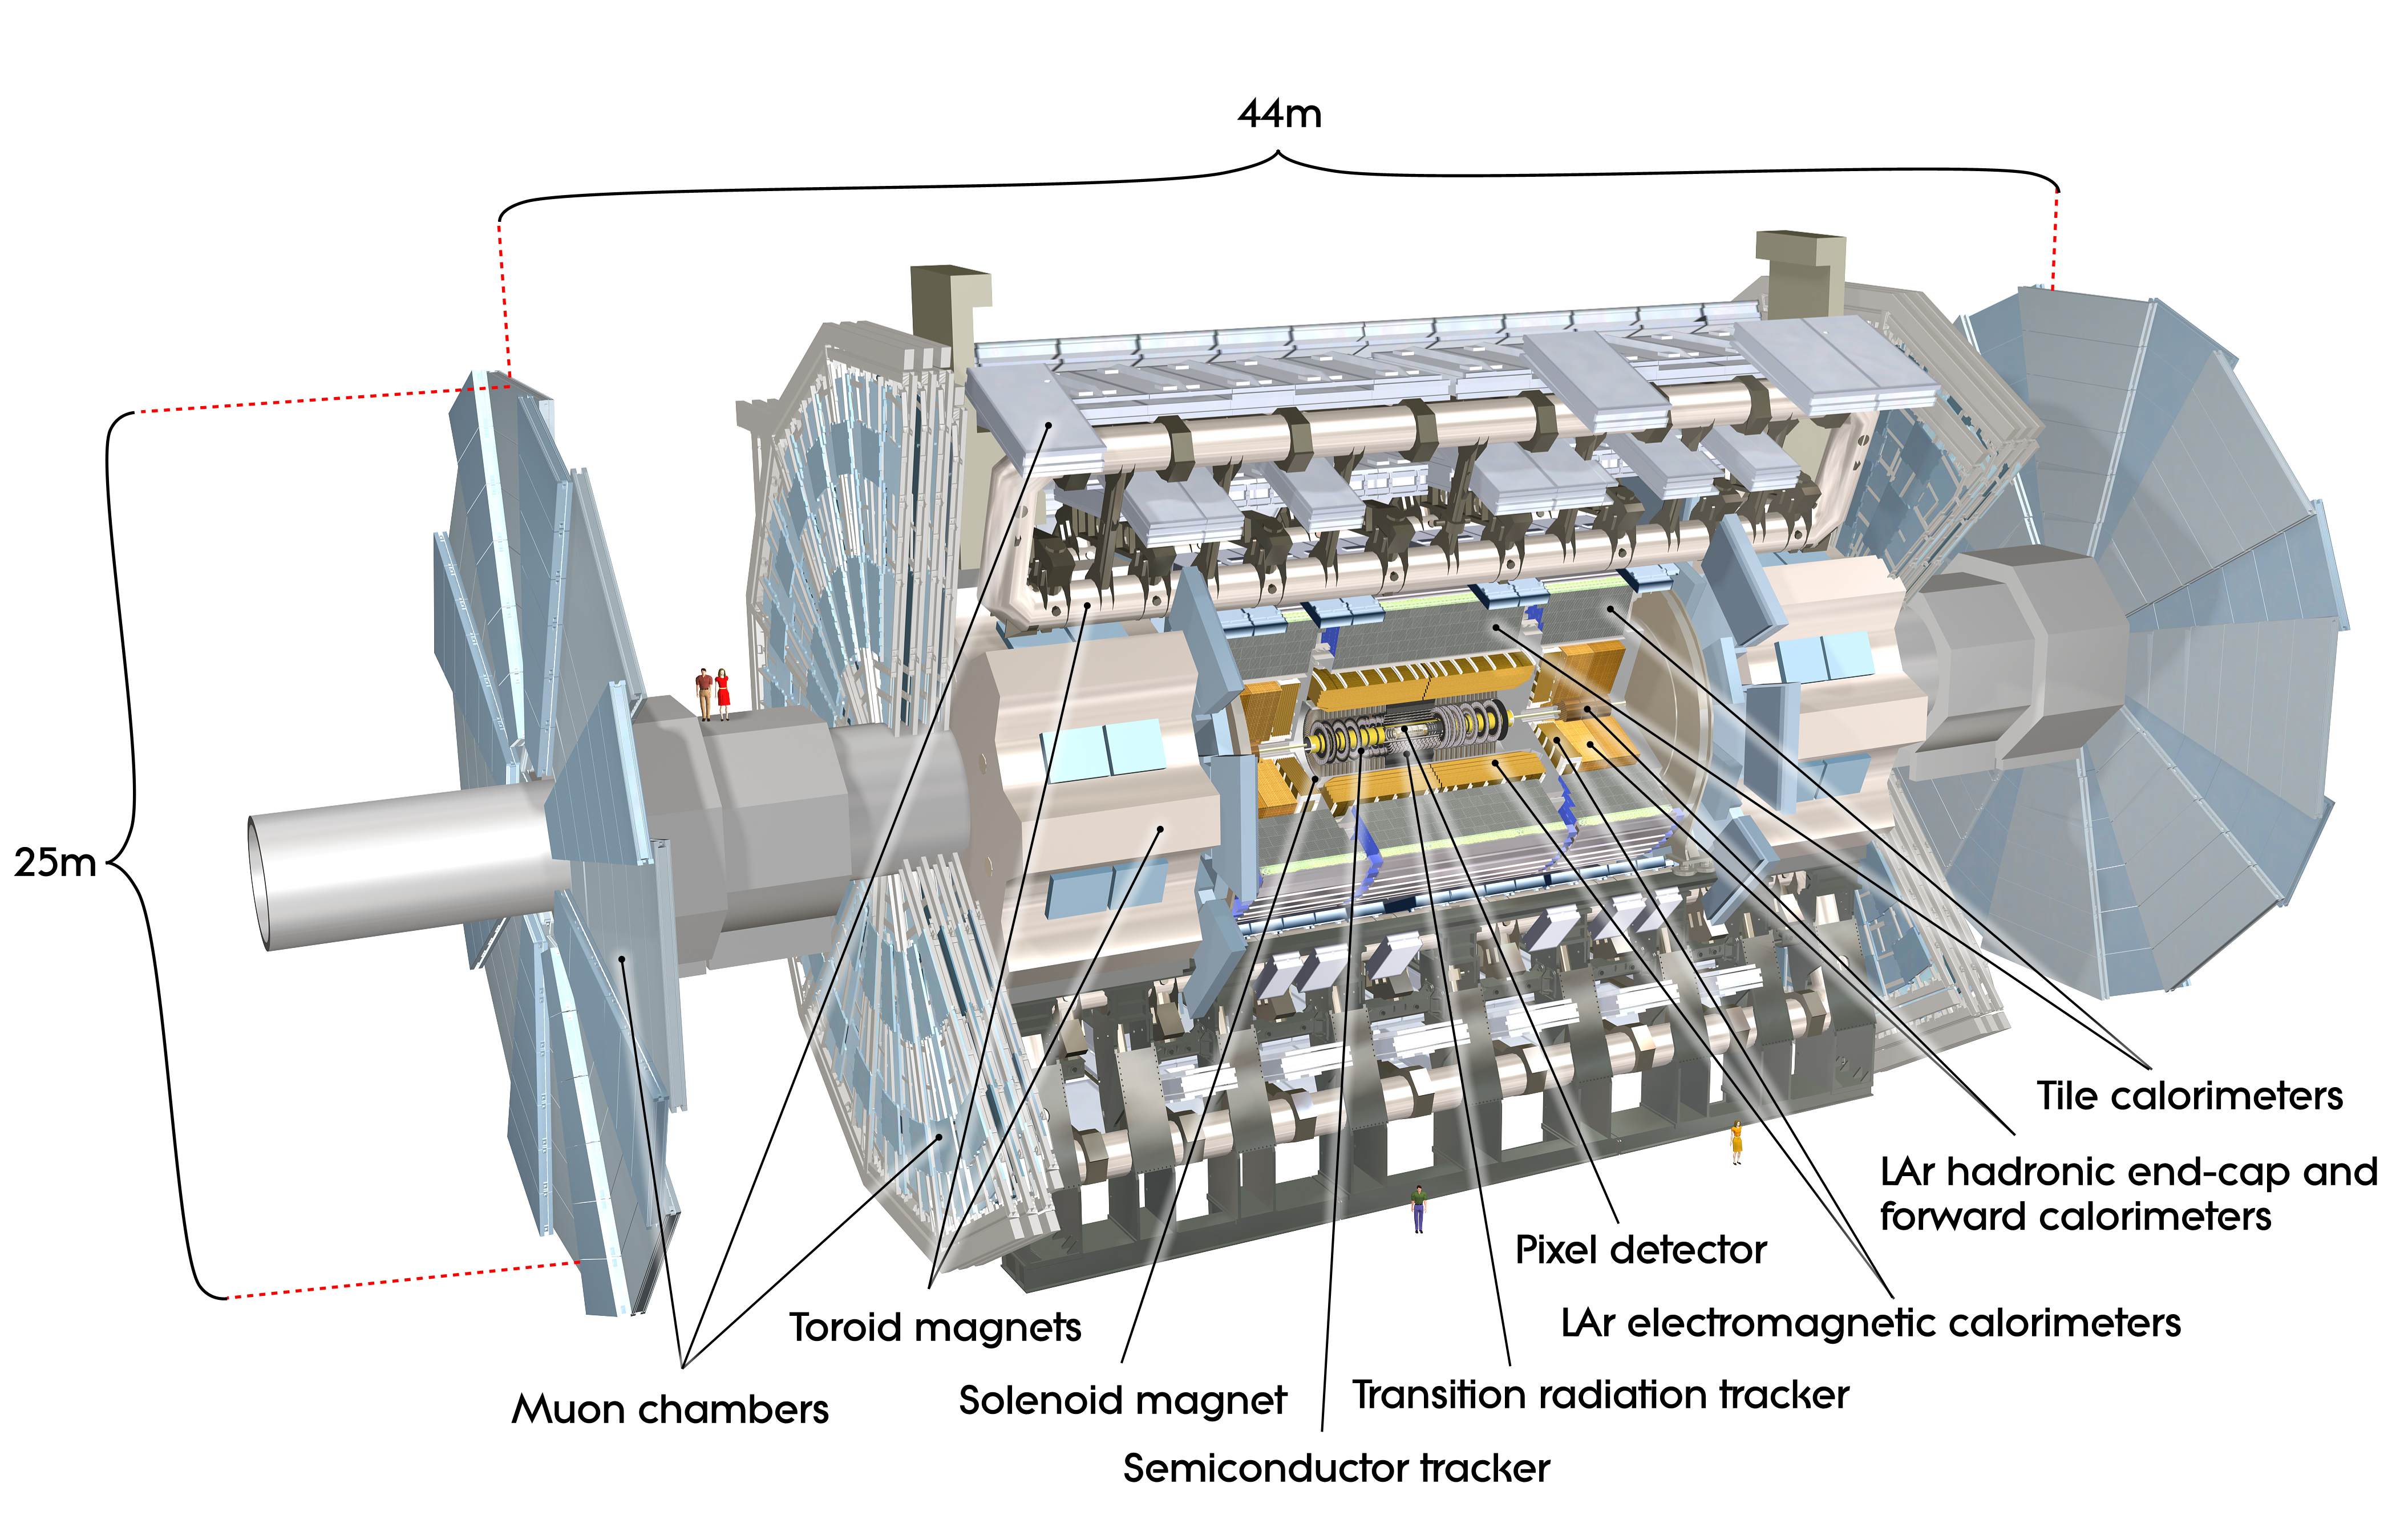
\includegraphics[width=0.9\textwidth]{atlas}
	\caption[The ATLAS detector]{Computer generated picture of the ATLAS detector, giving an overview on the various subsystems~\cite{Pequenao:1095924}.}
	\label{fig:atlas_detector}
\end{figure}